\subsection{Edades de los encuestados}
	\textbf{Tabla de Frecuencias:}
	Tabla que refleja las distribución de las respuestas de los encuestados ante los rangos de edades proporciados en la encuesta; muestra a su vez la frecuencia absoluta, frecuencia absoluta acumulada, frecuencia relativa(porcentual) y frecuencia relativa(porcentual) acumulada.
	
	%3ra pregunta del cuestionario, tabla de edades
	\begin{table}[h!]
		\centering
		\renewcommand{\arraystretch}{1.2} % Adjust this value to increase spacing
		\begin{tabular}{l c c c c}
			\hline
			{Rango de edad} & {\(f_i\)} & \textit{Fi} & \textit{hi}(\%) & \textit{Hi}(\%)\\
			\hline
			19 años o menos   & 39 & 39 & 50.65\% & 50.65\%\\
			20 - 23 años       & 20 & 59 & 25.97\% & 76.62\%\\
			24 - 27 años       & 8  & 67 & 10.39\% & 87.01\%\\
			28 años o más      & 10 & 77 & 12.99\% & 100\%\\
			\hline
			Total			   & 77 & & 100\% \\
			\hline
		\end{tabular}
		\caption{Distribución de respuestas por rango de edad}
		\label{tabla:edad}
	\end{table}
	
	\textbf{Media (\(\overline{x}\))}: Para el rango "19 años o menos" se ha tomado como referencia 17.5
	\begin{equation*}
		\overline{X} = \frac{\sum (x_i \cdot f_i)}{\sum f_i} = \frac{(17.5 \cdot 39) + (21.5 \cdot 20) + (25.5 \cdot 8) + (30 \cdot 10)}{77} \approx 20.99
	\end{equation*}
	% Formula y solución de la mediana
	\textbf{Mediana}:
	La mediana es el valor que divide el conjunto de datos en dos partes iguales. Con \(N = 77\), la mediana se encuentra en la posición:
	\begin{equation*}
		\text{Posición de la mediana} = \frac{N + 1}{2} = \frac{77 + 1}{2} = 39
	\end{equation*}
	Por lo tanto, la mediana corresponde a "Menos de 19 años".
	
	% Solución de la moda
	\textbf{Moda}: La moda es el valor con la mayor frecuencia, que en este caso es Menos de 19 años con \(f_i = 39\).

	\begin{figure}[H]
		\centering
		\hspace*{-1.5cm}
		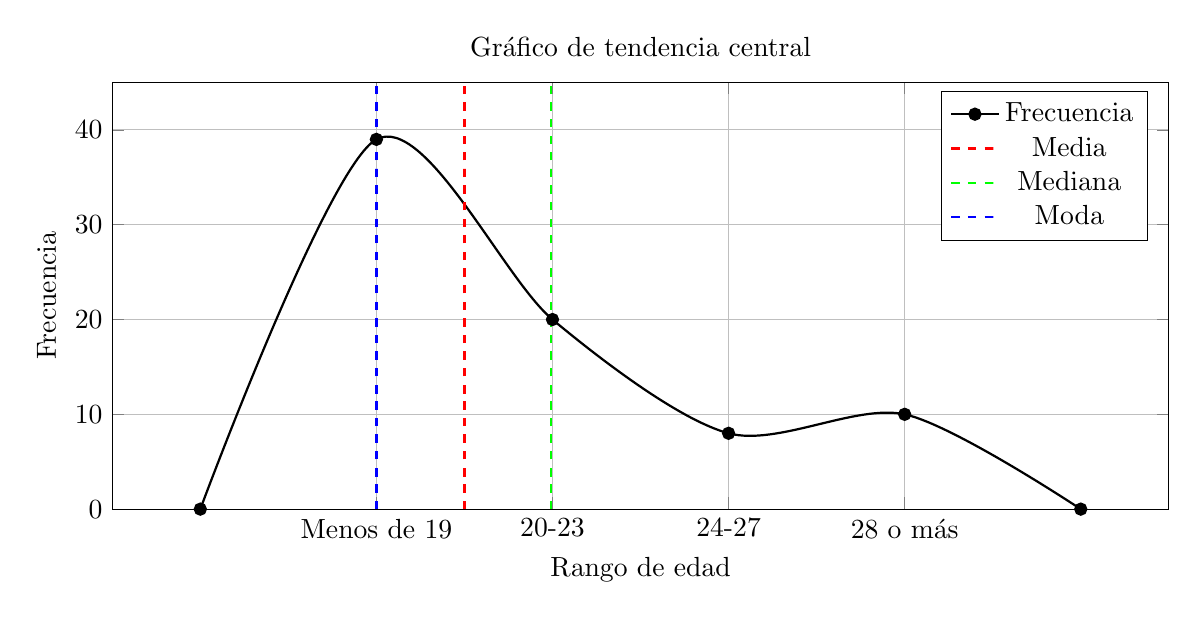
\begin{tikzpicture}
			\begin{axis}[
				width=15cm, height=7cm,
				xlabel={Rango de edad},
				ylabel={Frecuencia},
				xtick={1,2,3,4},
				xticklabels={Menos de 19, 20-23, 24-27, 28 o más},
				extra x ticks={1.5, 1.99},
				ymin=0, ymax=45,
				grid=major,
				smooth,
				tension=0.5,
				extra tick style={opacity=0},
				title={Gráfico de tendencia central} %Invisibiliza los ticks extra declarados
				]
				
				% Poligono de frecuencias
				\addplot[
				mark=*,
				color=black,
				thick
				] coordinates {
					(0,0)
					(1,39) % Menos de 19 años
					(2,20) % 20-23
					(3,8)  % 24-27
					(4,10) % 28 o más
					(5,0)
				};
				
				%Media
				\addplot[
				color=red,
				thick,
				dashed
				] coordinates {(1.5, 0) (1.5, 45)}; 
				%Mediana
				\addplot[
				color=green,
				thick,
				dashed
				] coordinates {(1.99, 0) (1.99, 45)};
				%Moda
				\addplot[
				color=blue,
				thick,
				dashed
				] coordinates {(1, 0) (1, 45)}; 
				\legend{Frecuencia, Media, Mediana, Moda}
			\end{axis}
		\end{tikzpicture}
		\caption{Gráfico de frecuencia con línea de tendencia}
	\end{figure}
	\textbf{Interpretación de resultados:}
	
	Se puede apreciar que la concentración de las edades está alrededor del rango de "menos de 19 años" dado que tanto la moda como la media pertenecen a este rango